\subsection{Model Validations}

The recreation of the figures of the respective publication of each model, is a common way to validate the new implementation. The following subsections show the results of the recreation and a short summary of what the figures entail. Additionally, the things that have worked or not, will be presented.

\subsubsection{Bellasio2019}

\begin{figure}
    \centering
    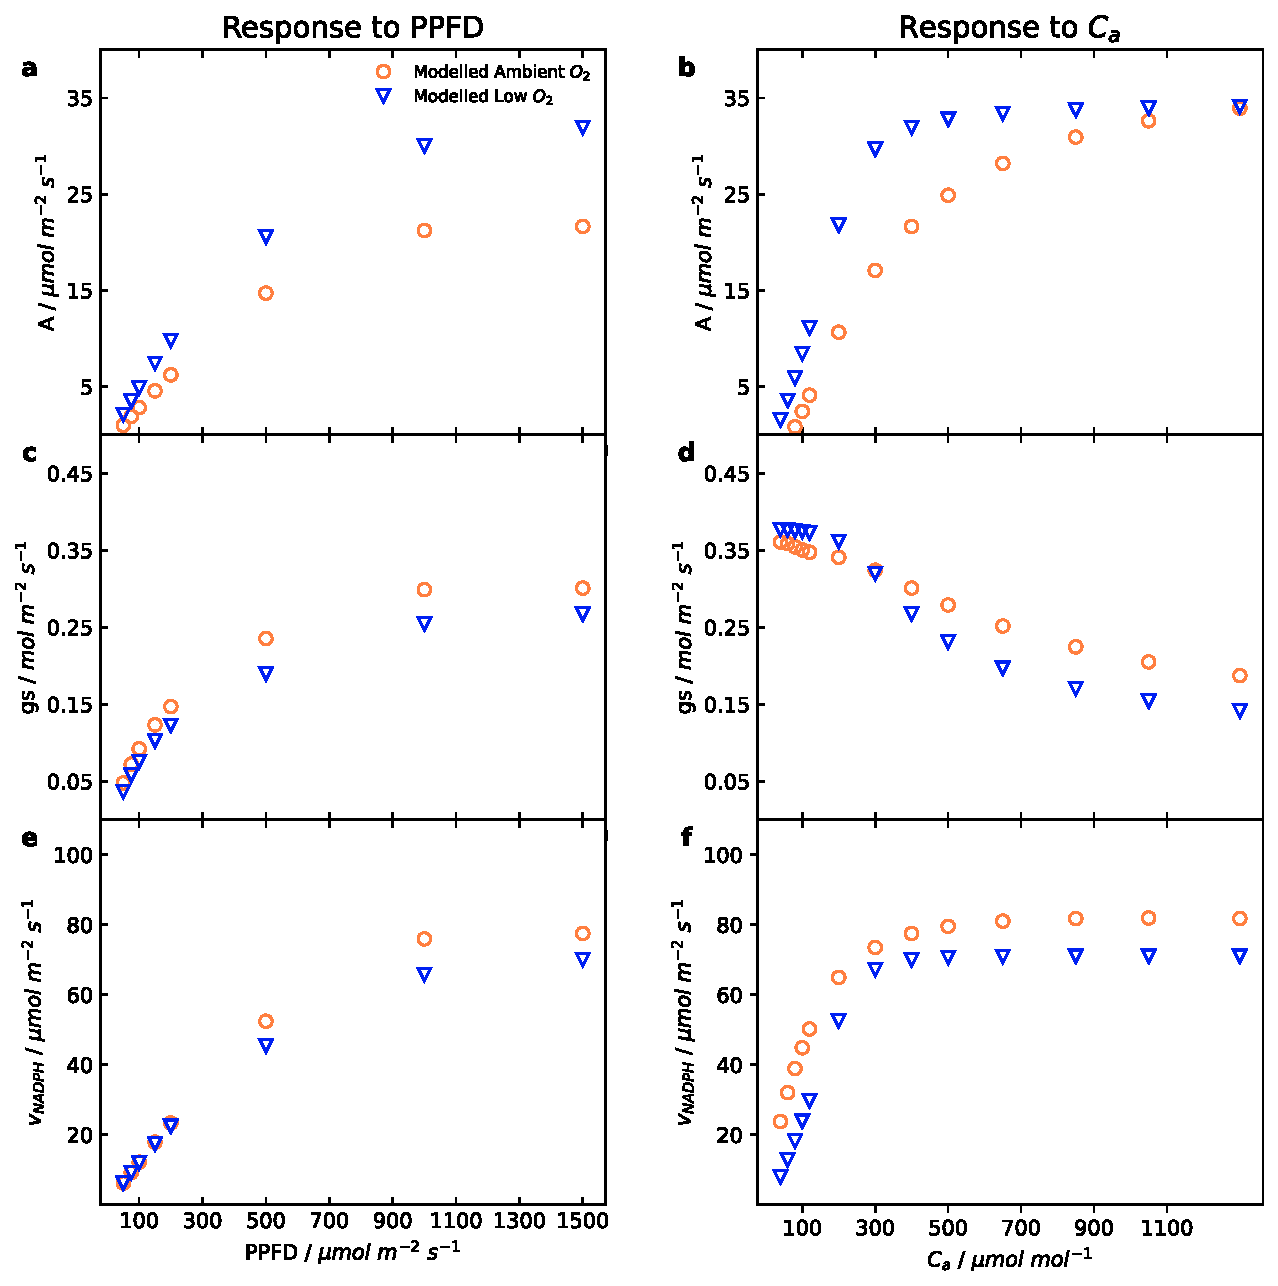
\includegraphics[width=0.7\textwidth]{Figures/Validations/bellasio2019_fig3.pdf}
    \captionprof{Simulated \glsentryshort{A}-\glsentryshort{ppfd} and \glsentryshort{A}-\glsentryshort{ca} response curves. Figure 3 of the Bellasio2019 model.}{test} 
\end{figure}

\begin{figure}
    \centering
    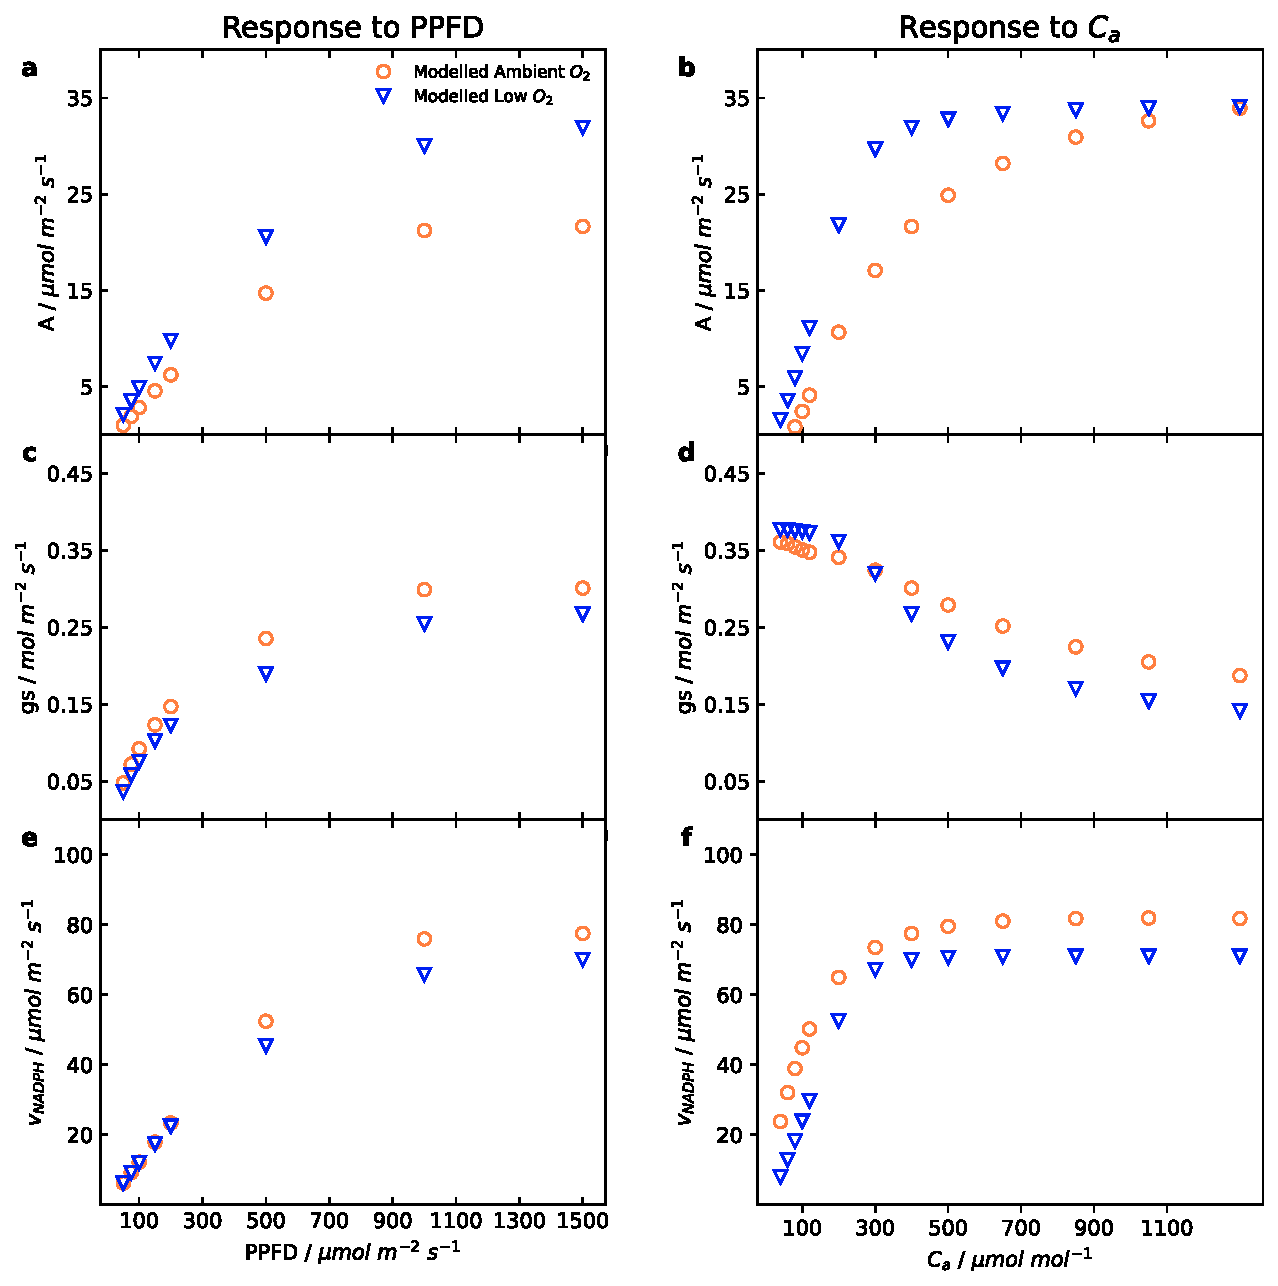
\includegraphics[width=0.7\textwidth]{Figures/Validations/bellasio2019_fig3.pdf}
    \captionprof{Figure 3 of the Bellasio2019 model. }{test} 
\end{figure}

\subsubsection{Fuente2024}

\subsubsection{Li2021}

\subsubsection{Matuszynska2016}

\subsubsection{Saadat2021}

\subsection{Model Demonstrations}

\subsubsection{Daylight Simulation}

\begin{figure}
    \centering
    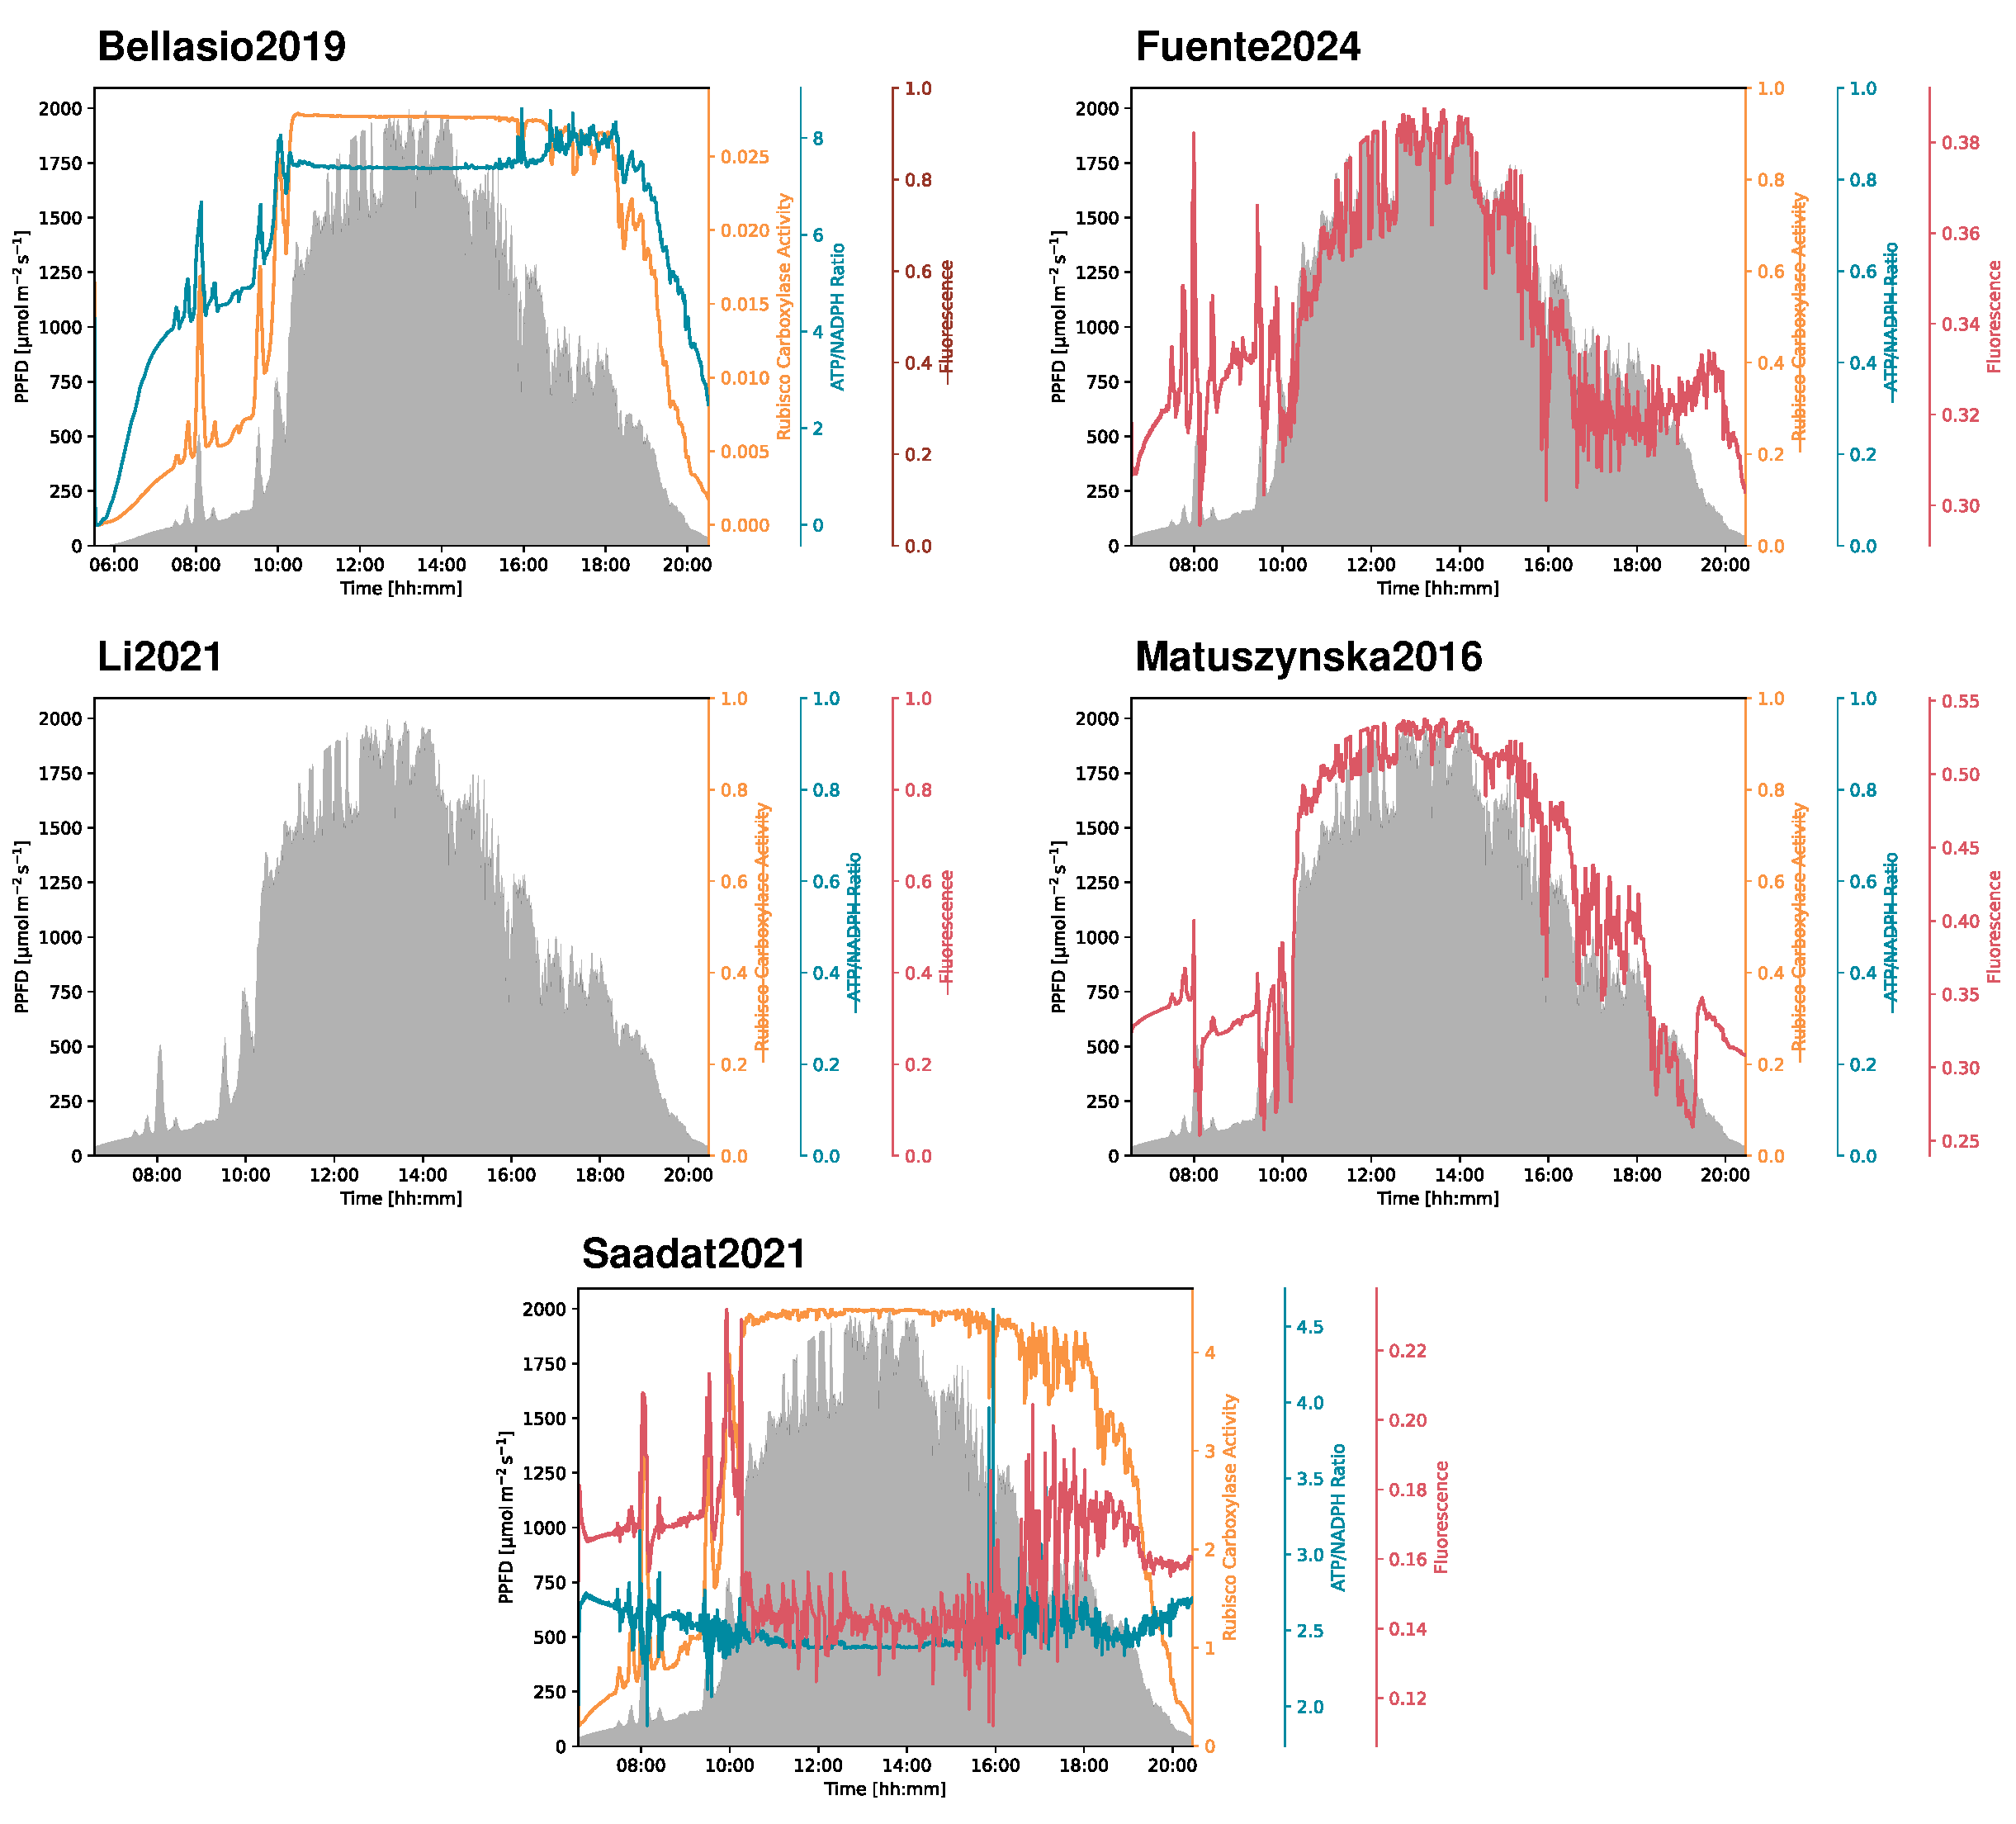
\includegraphics[width=0.7\textwidth]{Figures/Demonstrations/daysimulation.pdf}
    \captionprof{Combined Daylight Simulation demonstrations of all models.}{Sample simulation of a day cycle using real \glsentryfull{ppfd} data from Kansas, USA on June 19, 2023. The data was obtained from the \glsentryfull{neon} data portal~\cite{nationalecologicalobservatorynetworkneonPhotosyntheticallyActiveRadiation2023} and is used to create a protocol for the light intensity \glsentryshort{ppfd} over the course of the day, in a minute interval. The data used is filtered to only show a \glsentryshort{ppfd} that equals or is higher than \qty{40}{\micro\mol\per\square\meter\per\second}. This threshold is chosen as it has shown to allow most models to still simulate the photosynthetic machinery, while still being a decent representation of the actual daylight conditions. The simulation is run using the default parameters and initial conditions of each model, and the \glsentryfull{vc}, \glsentryfull{atp} and \glsentryfull{nadph} ratio, and \glsentryfull{F} results is plotted over the course of the day, if possible. The results do not represent actual plant behavior, but show the capabilities of the model to simulate complex and more realistic light protocols. In Bellasio2019~\cite{bellasioGeneralisedDynamicModel2019}, only } 
\end{figure}

\subsubsection{FvCB Add-on}
\begin{figure}
    \centering
    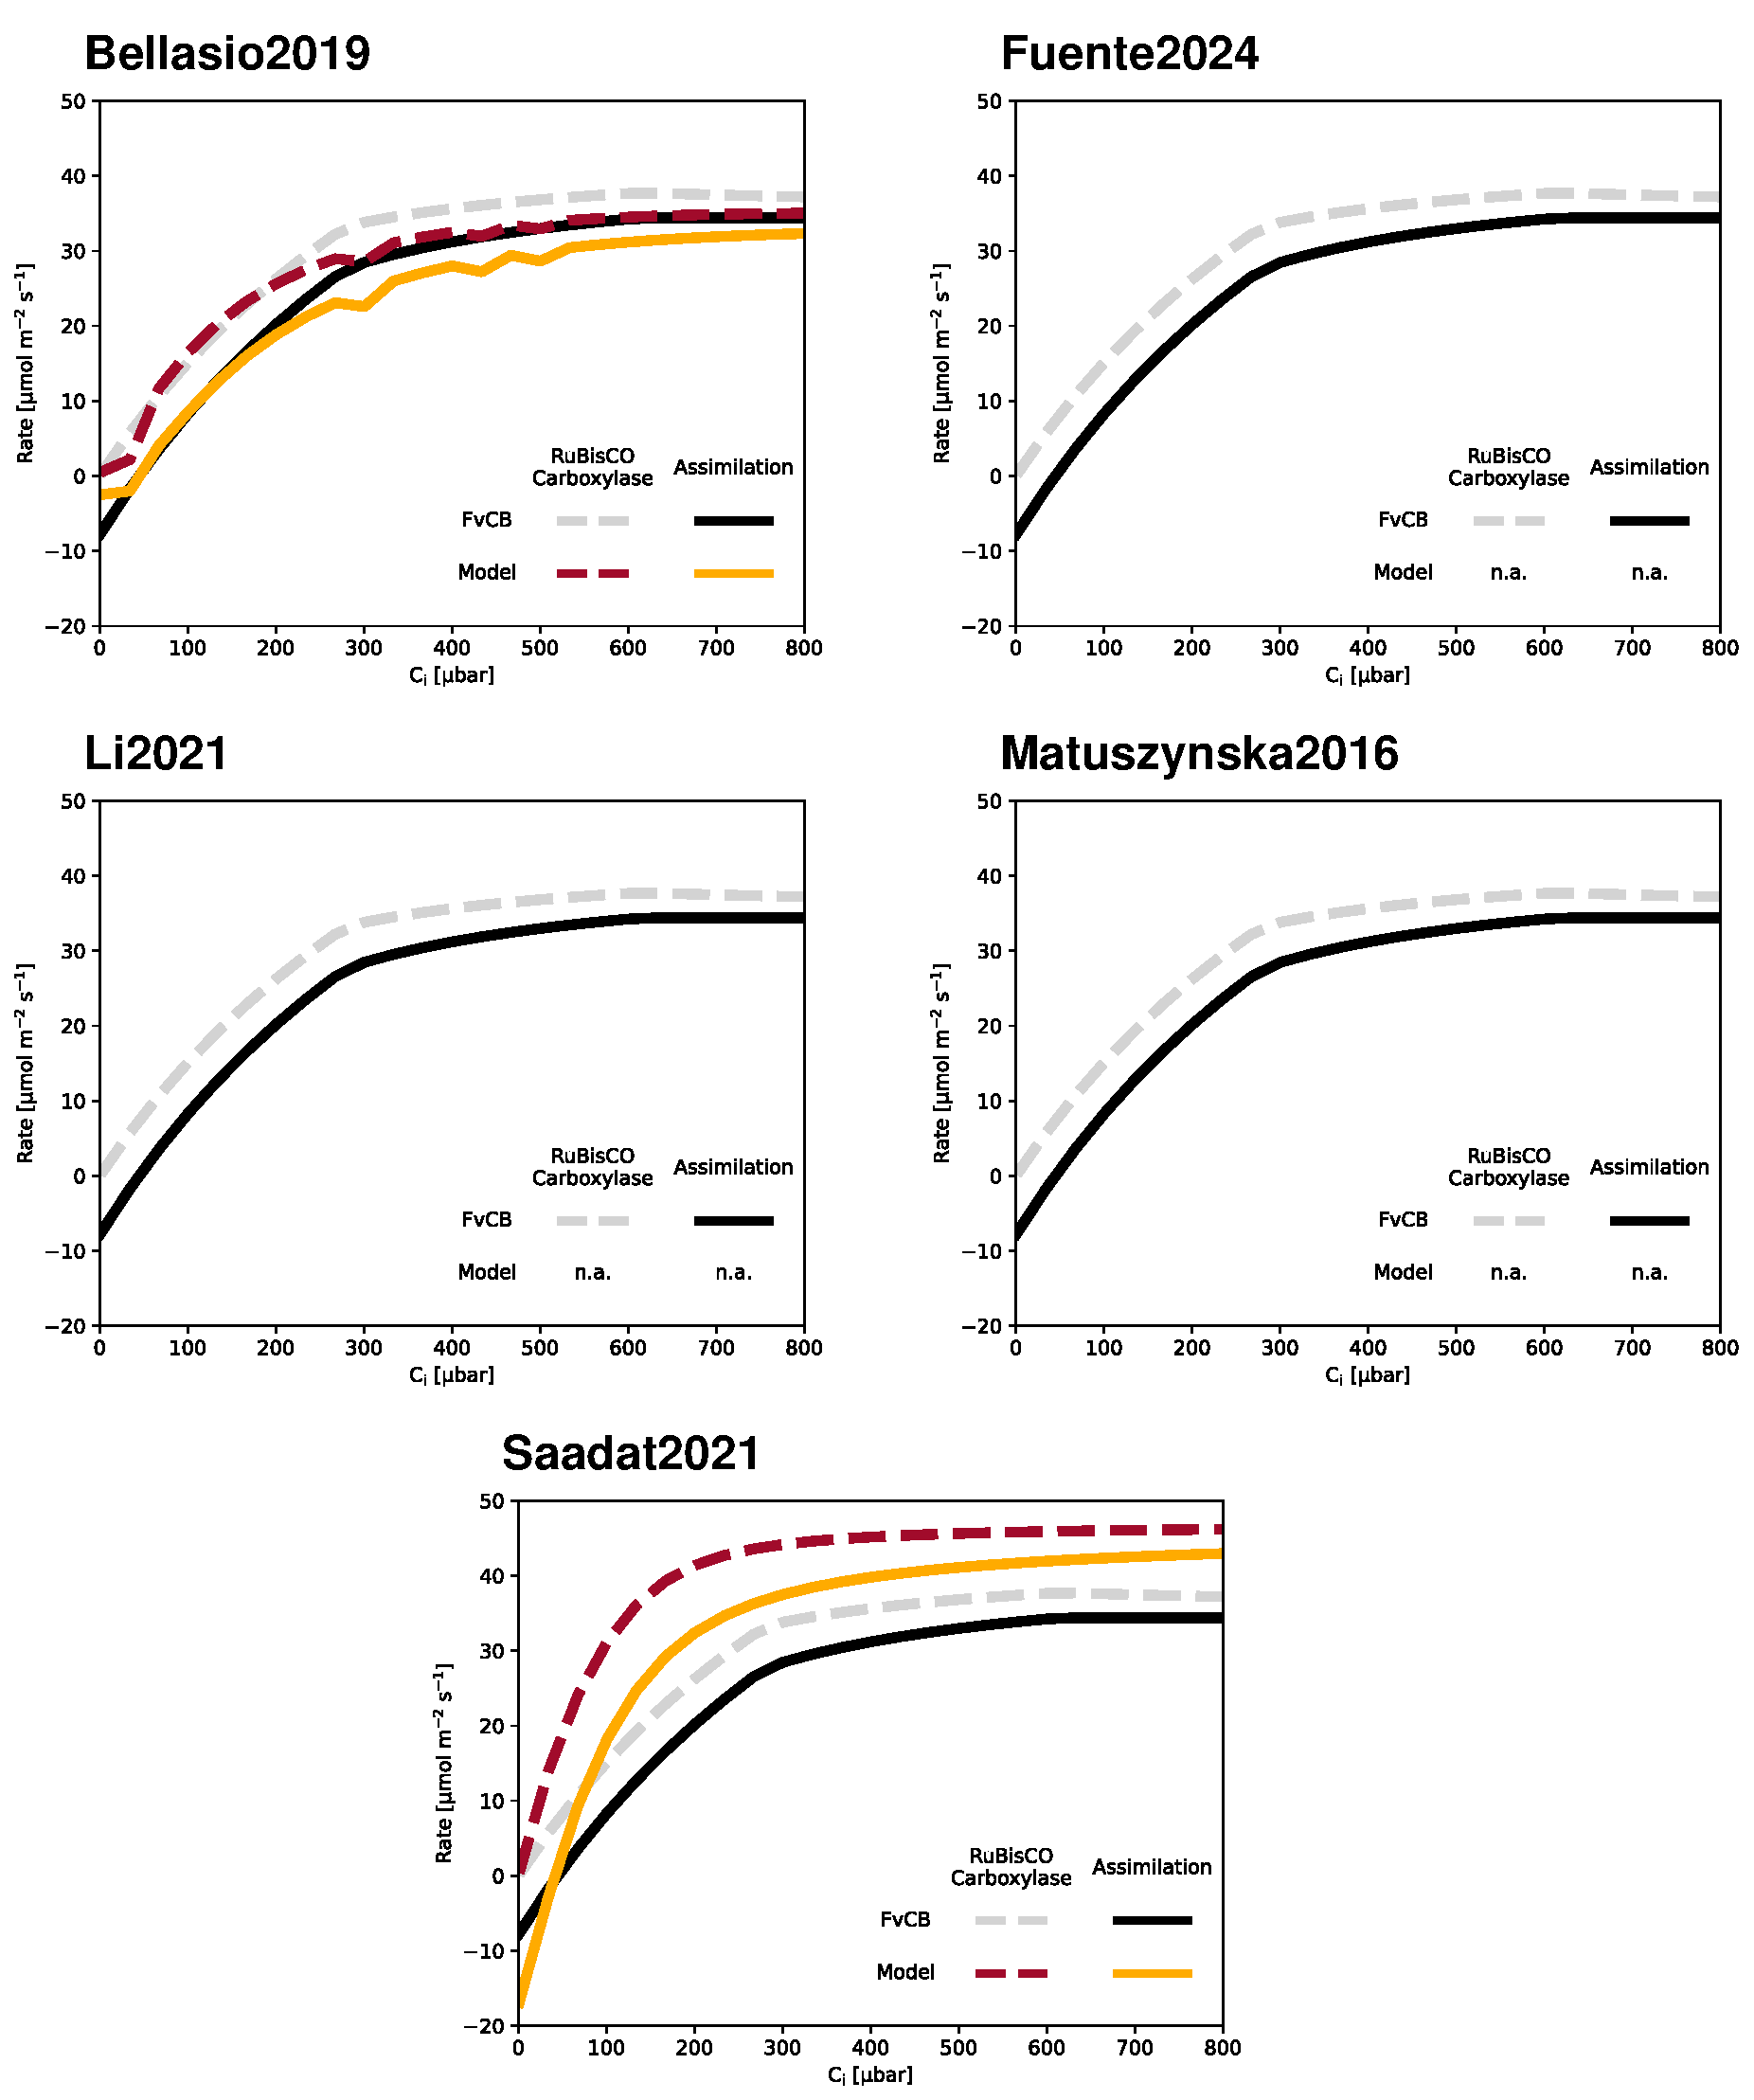
\includegraphics[width=0.7\textwidth]{Figures/Demonstrations/fvcb.pdf}
    \captionprof{Combined FvCB Addon demonstrations of all models.}{Comparison of modelled \glsentryfull{A} and \glsentryfull{vc} against the \glsentryfull{fvcb} model. The \glsentryshort{fvcb} model is calculated using the min-W approach as described by Lochoki and McGrath (2025)~\cite{lochockiWidelyUsedVariants2025a}. To be able to simulate \glsentryshort{A}, there are two mandatory quantities that need to be present in the model: \glsentryfull{co2} concentration and \glsentryshort{vc}. If one of these parameters is missing, the \glsentryshort{fvcb} model will still be shown, but no comparison with the model will be possible. Other parameters that are required to calculate the \glsentryshort{fvcb} model will be added as parameters with default values if they are not present in the model. The simulation is then run until steady-state, or quasi-steady-state if not otherwise possible, for different \glsentryfull{ci} partial pressure. The carbon assimilation shown does not represent actual values but rather a theoretical curve to compare the kinetic model to the popular \glsentryshort{fvcb} model.} 
\end{figure}

\subsubsection{Standard PAM Simulation}

\begin{figure}
    \centering
    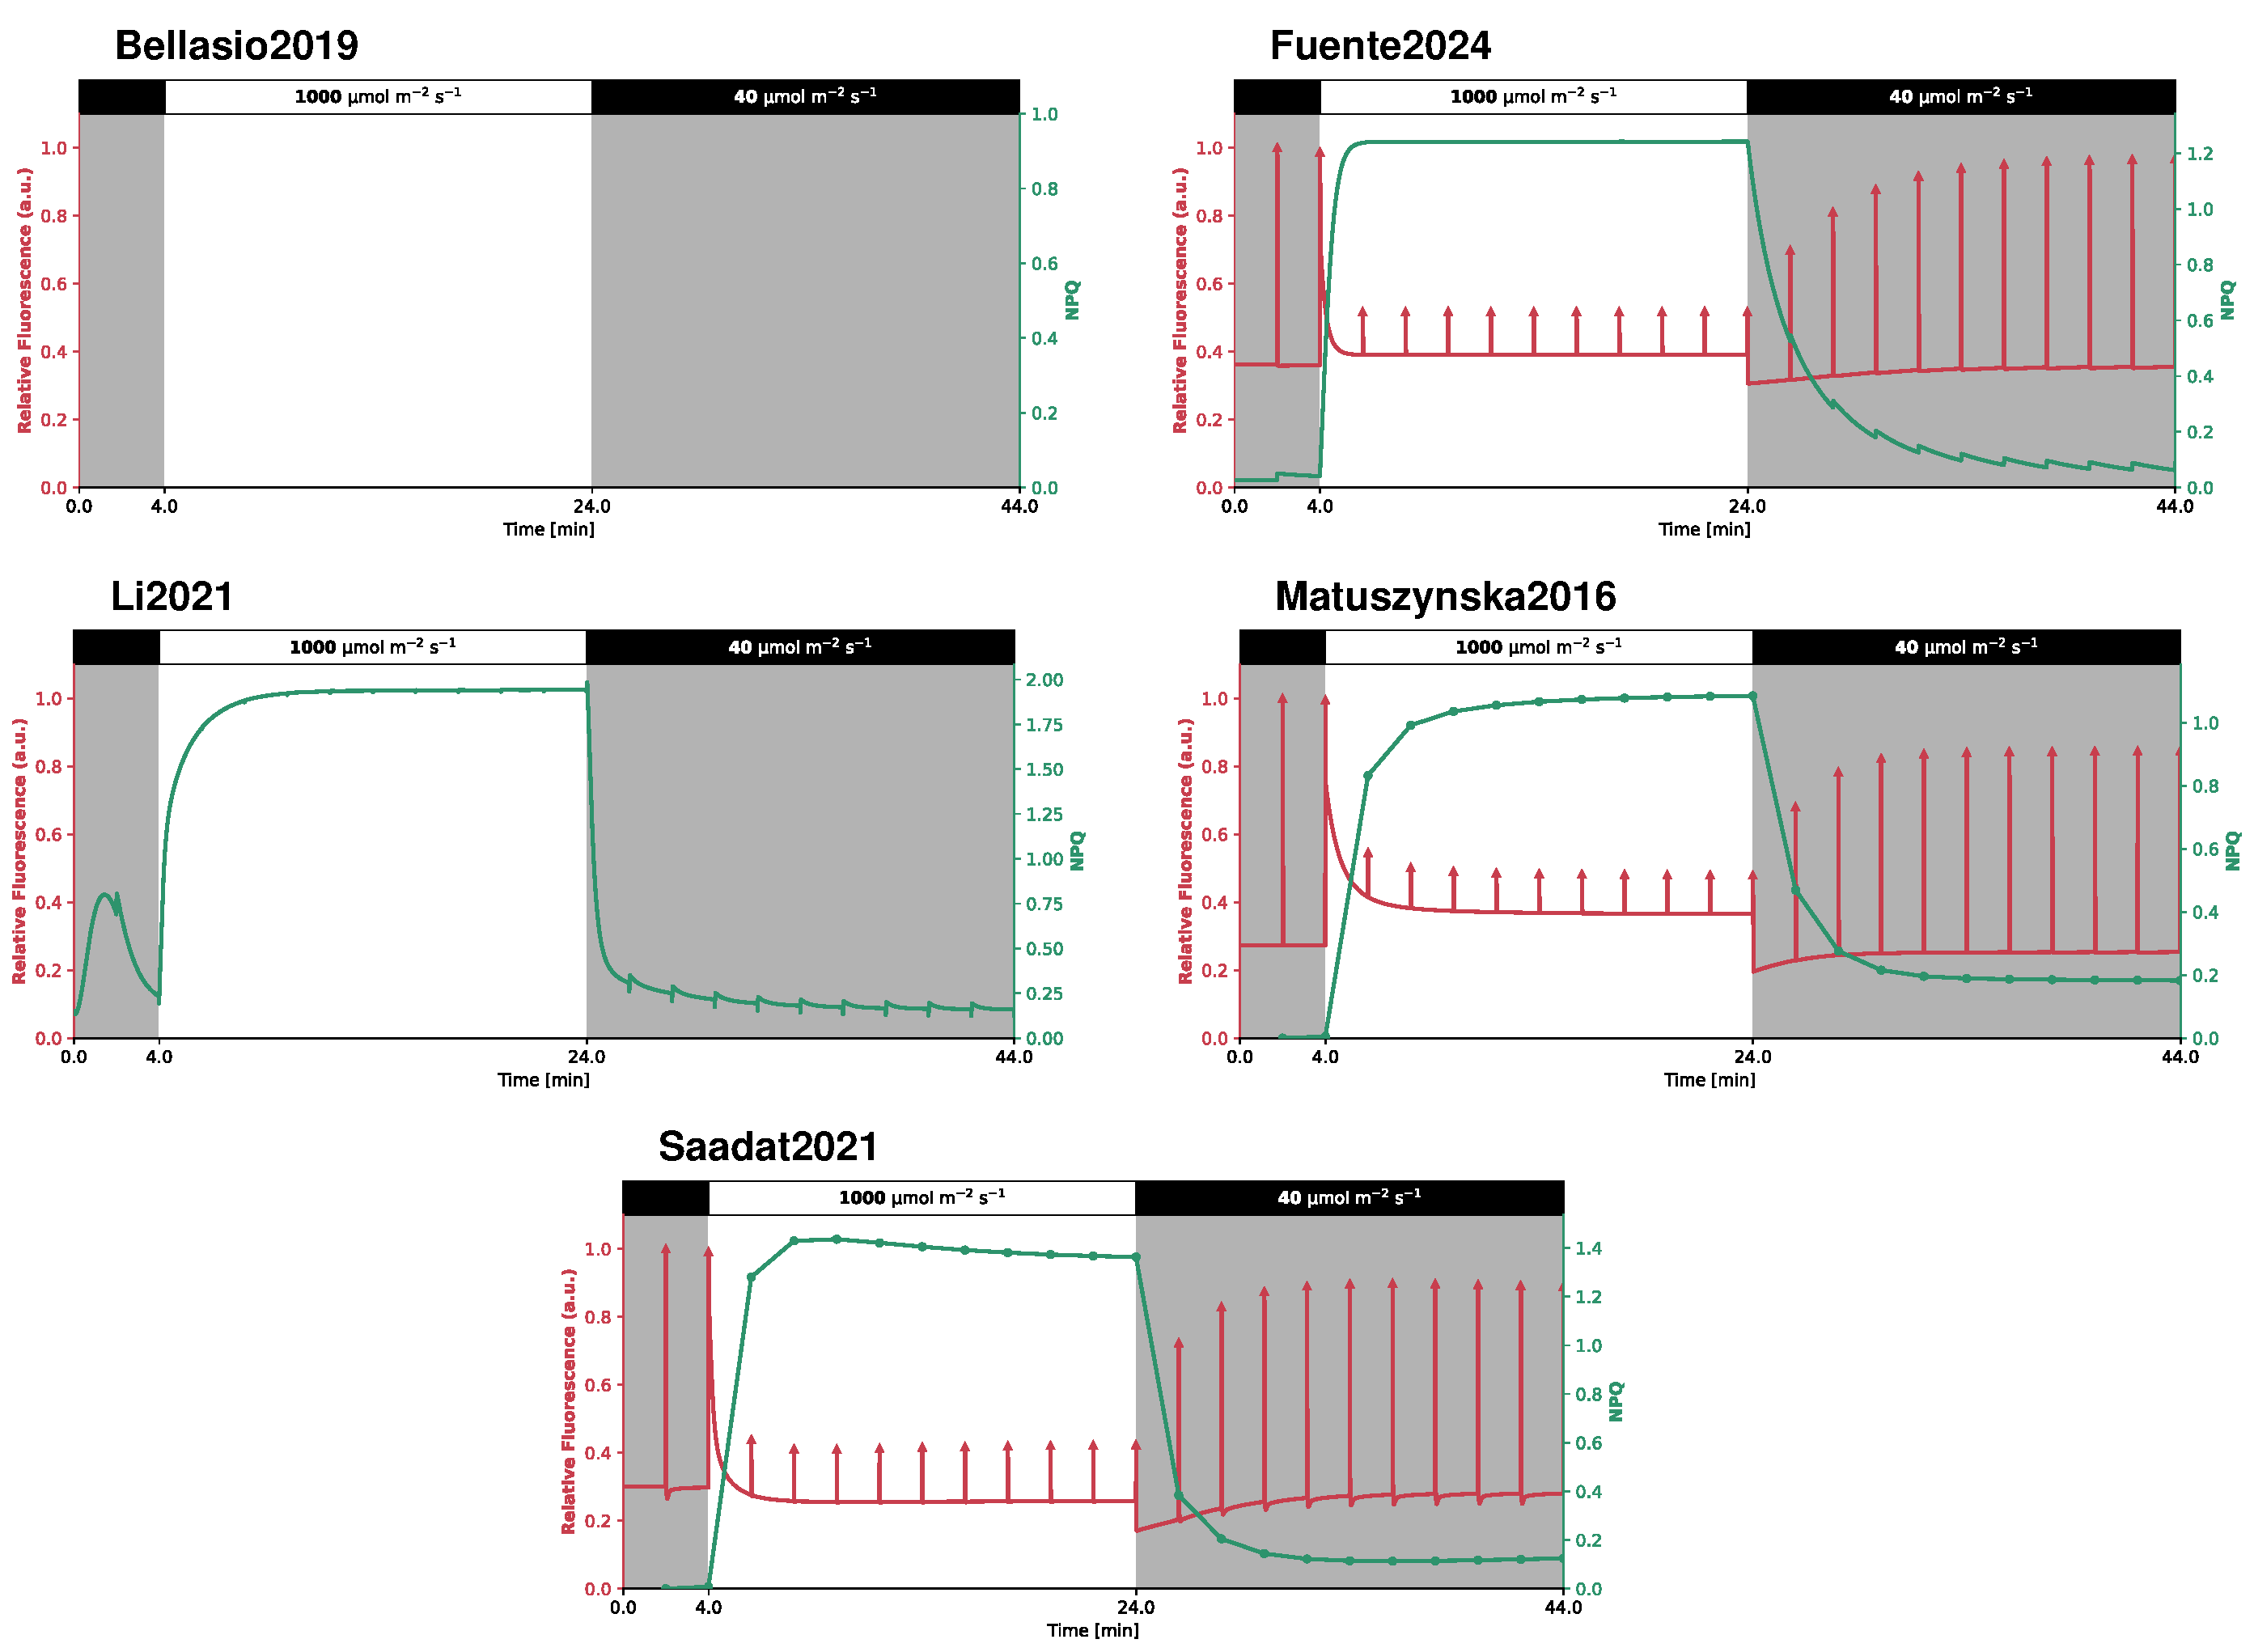
\includegraphics[width=0.7\textwidth]{Figures/Demonstrations/pam.pdf}
    \captionprof{Combined PAM Simulation demonstrations of all models.}{Sample simulation of a common \glsentryfull{pam} protocol to show fluctuations of \glsentryfull{F} and \glsentryfull{npq} using saturating pulses. The simulation protocol is as follows: A dark adaptation period that simulates for 30 minutes at a dark light intensity (\qty{40}{\micro\mol\per\square\meter\per\second}), then the actual protocol starts. The protocol consists of 22 periods with each being 2 minutes of length. That period consists of a specific light intensity of the respective type of period and ends with a saturating pulse with a length of \qty{0.8}{s} and a light intensity of \qty{3000}{\micro\mol\per\square\meter\per\second}. First, two dark periods with light intensity of \qty{40}{\micro\mol\per\square\meter\per\second}, followed by ten light periods with light intensity of \qty{1000}{\micro\mol\per\square\meter\per\second}, then ten dark periods again. The simulation is run using the default parameters and initial conditions of each model.} 
\end{figure}

\subsubsection{MCA of Photosynthesis}

\begin{figure}
    \centering
    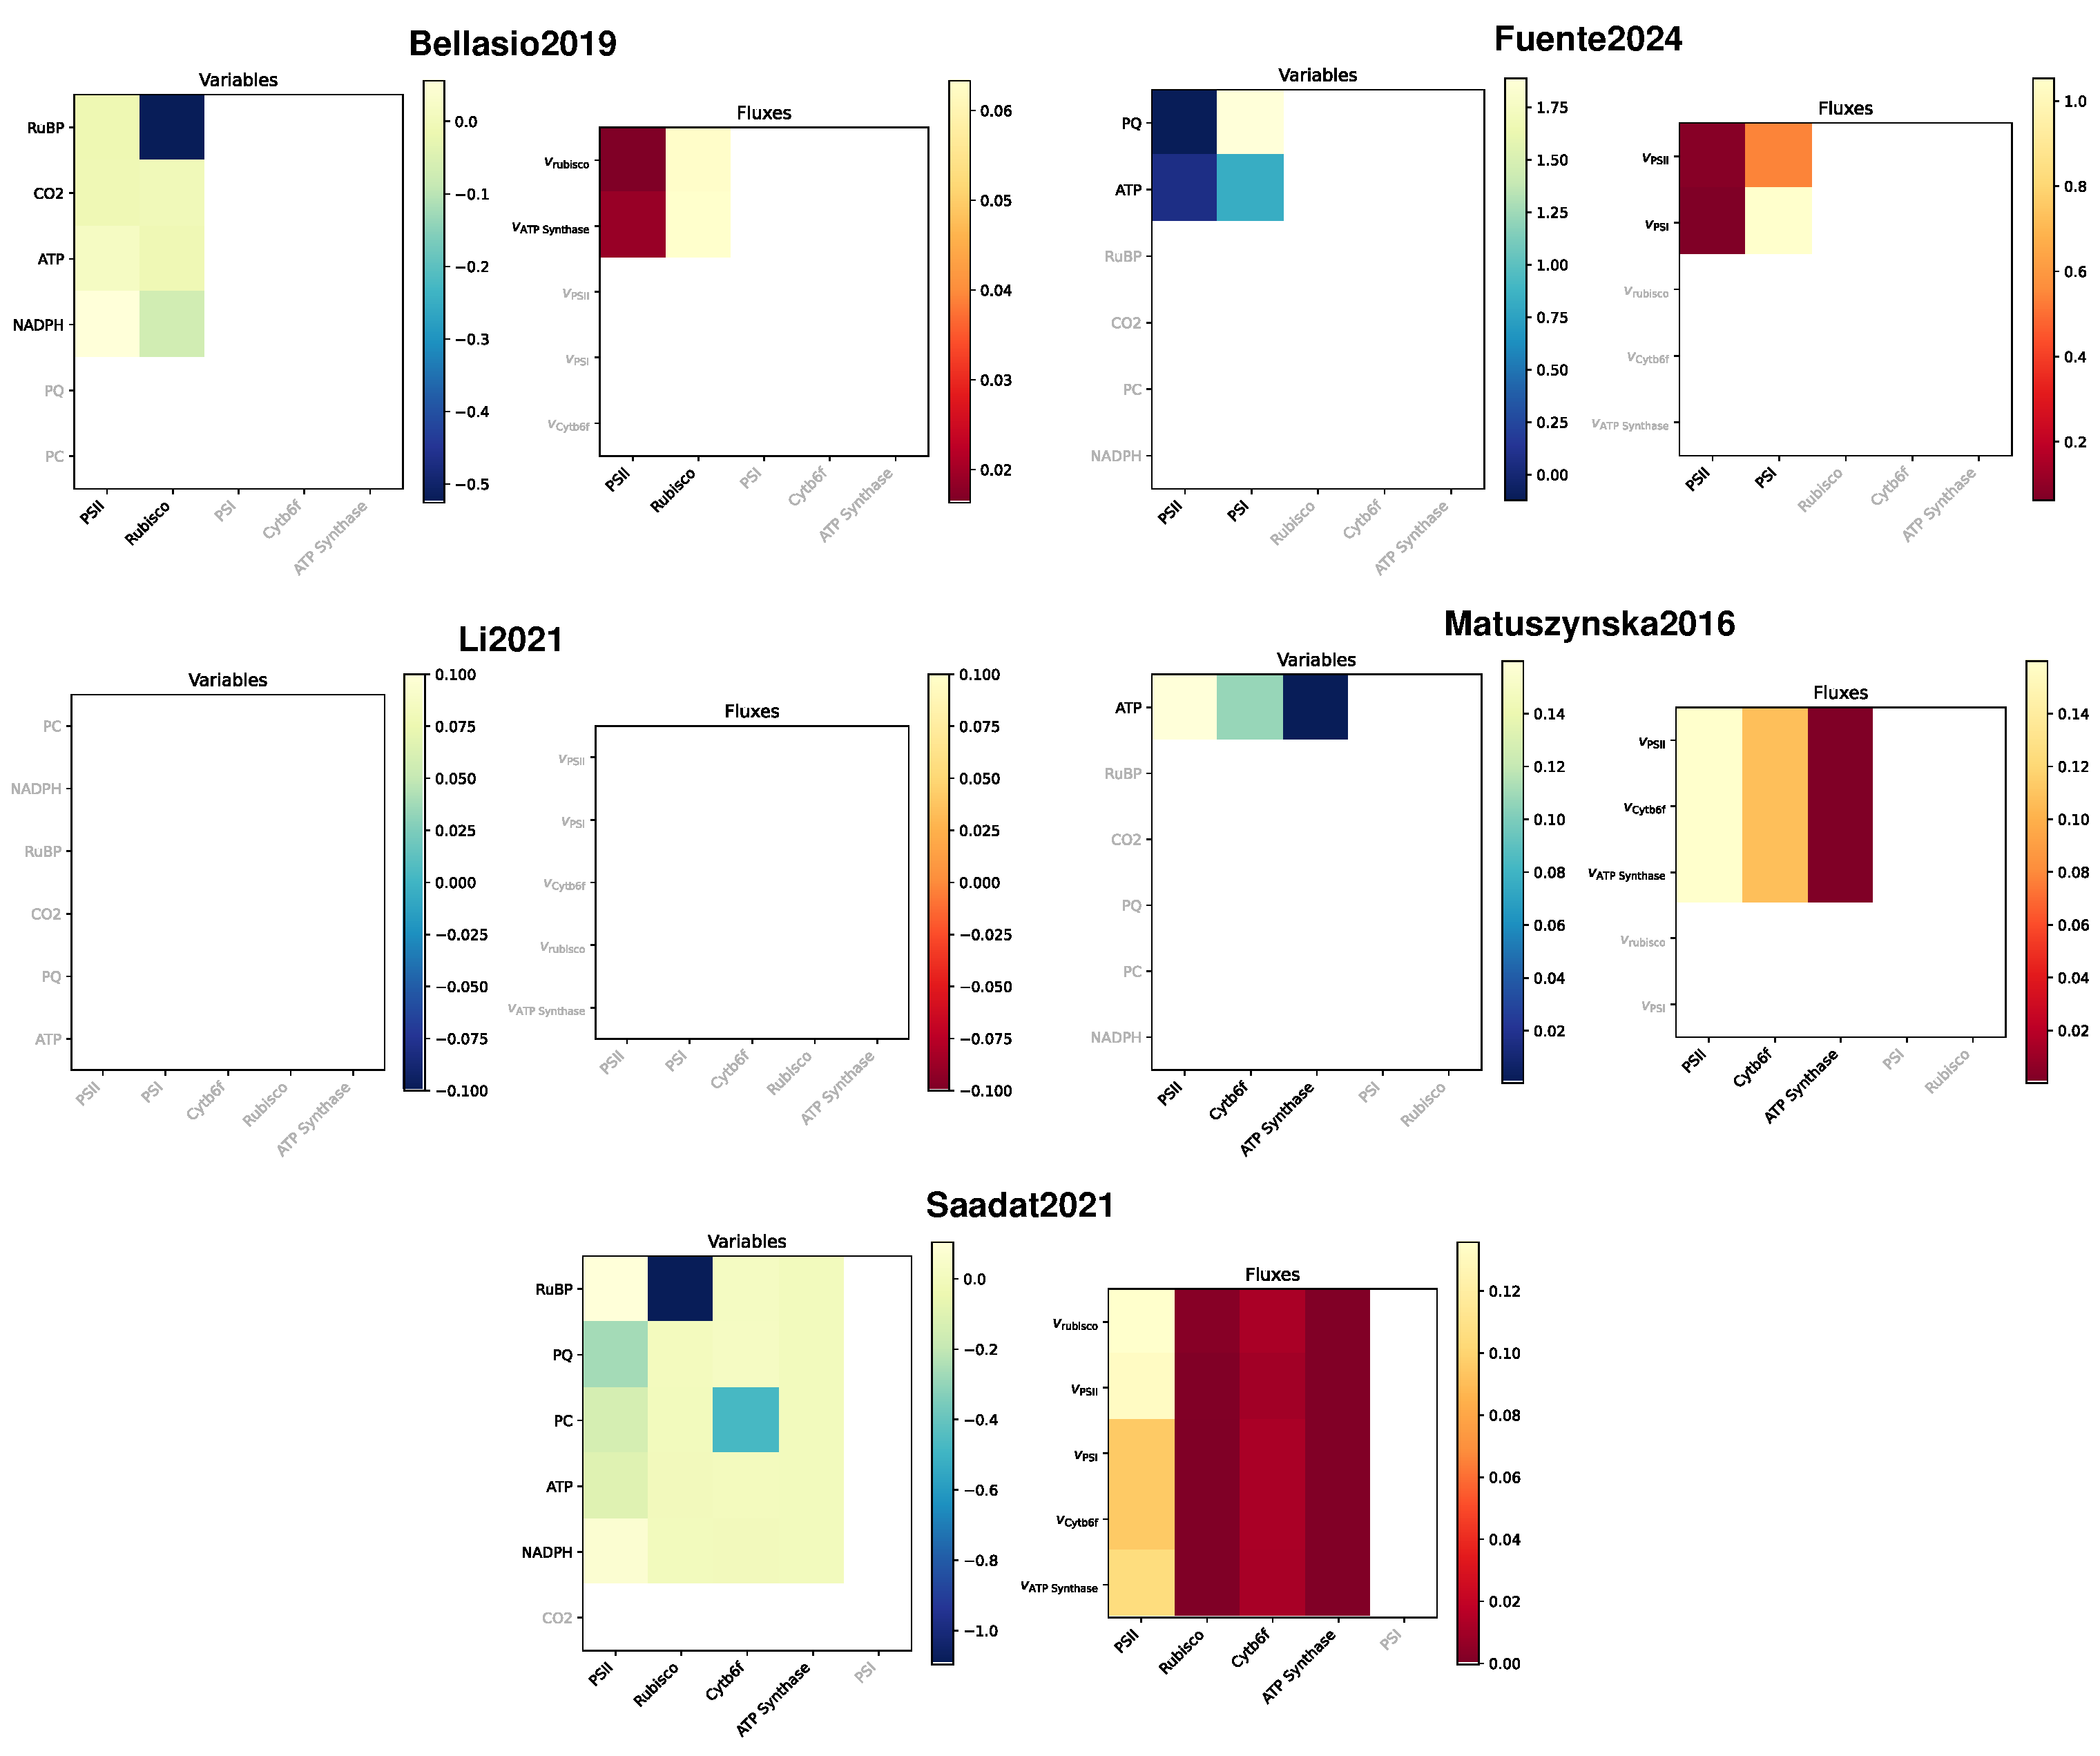
\includegraphics[width=0.7\textwidth]{Figures/Demonstrations/mca.pdf}
    \captionprof{Combined MCA of Photosynthesis demonstrations of all models.}{A sample \glsentryfull{mca} of typical photosynthesis variables and fluxes. A control coefficient analysis is to be performed, therefore each parameter represents a single coefficient of the photosynthesis rate. The rates chosen should represent \glsentryfull{vc}, \glsentryfull{vpsii}, \glsentryfull{vpsi}, \glsentryfull{vb6f} and \glsentryfull{vatp}. The variables chosen should represent \glsentryfull{co2} concentration, \glsentryfull{rubp}, \glsentryfull{pq_ox}, \glsentryfull{pc_ox}, \glsentryfull{atp}, and \glsentryfull{nadph}. For each parameter to be scanned, the model is simulated to steady-state, with a displacement of $\pm 0.01\%$ of each respective parameter. The control coefficients are then calculated for each variable and flux by the following formula: $C_{{p}}^{{x}} = \frac{{x_\mathrm{{upper}} - x_\mathrm{{lower}}}}{{2 \cdot \mathrm{{disp}} \cdot p}}$, where $C_{{p}}^{{x}}$ is the control coefficient of parameter $p$ on variable or flux $x$, and $\mathrm{{disp}}$ is the displacement value. $x_\mathrm{{upper}}$ and $x_\mathrm{{lower}}$ are the steady-state result of $x$ at either $+\mathrm{{disp}}$ and $-\mathrm{{disp}}$ respectively. It has to be noted that the \glsentryshort{mca} results can be very dependent on the other values of the parameters in the model, therefore the results shown here are only representative of the default parameter set of the model.} 
\end{figure}

\subsubsection{Fitting of NPQ}

\begin{figure}
    \centering
    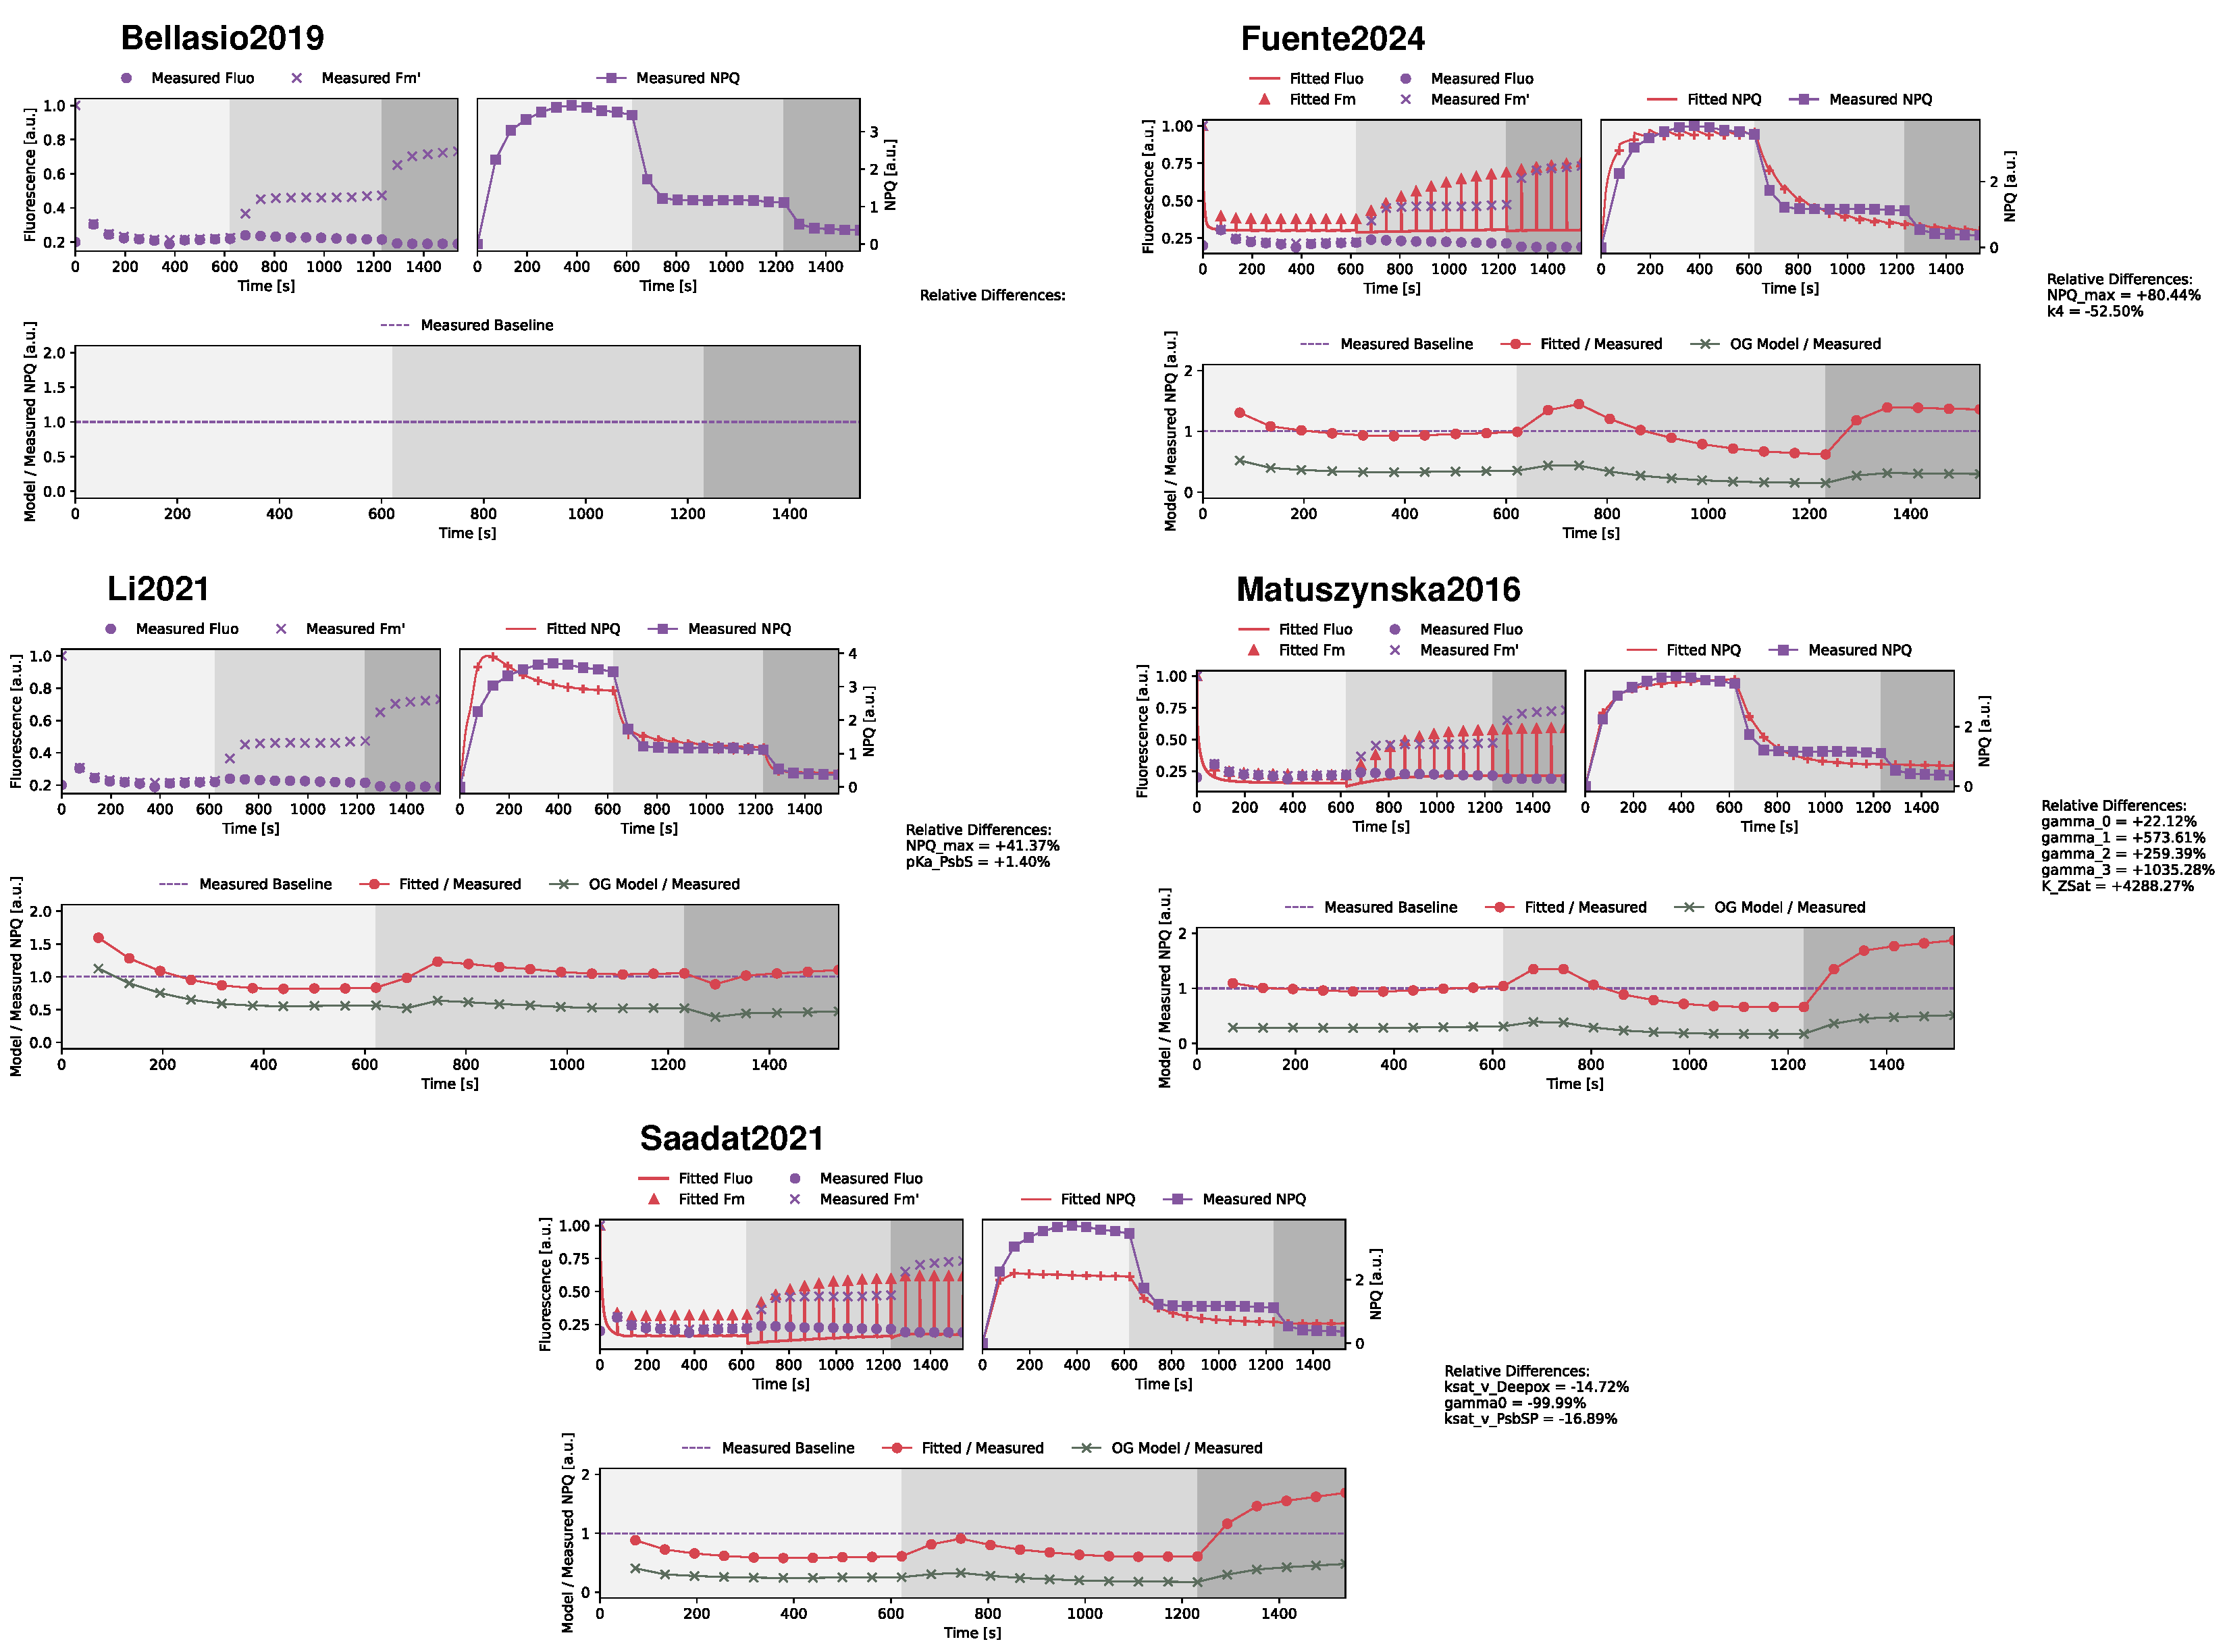
\includegraphics[width=\textwidth]{Figures/Demonstrations/fitting.pdf}
    \captionprof{Combined Fitting of NPQ demonstrations of all models.}{Sample fitting to experimental \glsentryfull{npq} data. The \glsentryshort{npq} data used is taken from experimental work published in von Bismarck (2022)~\cite{vonbismarckLightAcclimationInteracts2023} and was acquired using Maxi Imaging-PAM (Walz, Germany) using Col-0 \glsentryfull{arabidopsis} plants. It is assumed that the experiment follows the default \glsentryshort{pam} protocol of the machine, as no other experimental protocol has been given. Therefore, the protocol of each simulation follows the data given, where the length of one saturating pulse is set to \qty{720}{\micro\second} at a light intensity of \qty{5000}{\micro\mol\per\square\meter\per\second}. The light protocol consists of a dark adaptation period of 30 minutes to acclimate the simulation conditions. Then the actual protocol starts with a longer phase of high actinic light (\qty{903}{\micro\mol\per\square\meter\per\second}) for approximately 10 minutes, followed by a lower actinic light of (\qty{90}{\micro\mol\per\square\meter\per\second}) for 10 minutes, and then 5 minutes of a dark period. During each phase, saturating pulses are given approximately every 60 seconds. As the experimental data also provides exact time points for each pulse, these were taken as reference for the protocol and not the general time intervals. In the experimental work, the dark period consists of actual darkness, whereas in the simulation a low light intensity of \qty{40}{\micro\mol\per\square\meter\per\second} is used to avoid numerical issues. The fitting is performed using the \texttt{lmfit} package in Python with the leastsquare method. On top of that, a standard scaling towards the experimental data is done, to keep the fitting results in the same order of magnitude. To help the fitting converge, weights are applied to the data points, which are defined as the reciprocal of the standard deviation. These settings set are not to be taken as set in stone, as fitting is a highly experimental process and differing settings might be required depending on the model and data used. These settings are a basic starting point for fitting data to a model. The hardest and most impactful decision while fitting is the choice of parameters to fit. There are many ways to find which parameters may be most impactful to fit, such as sensitivity analysis or metabolic control analysis. However, either way experimenting with different parameter sets is always required to find the best fitting practice, which differs for each model and also data to fit to.} 
\end{figure}

\subsection{Website}